%\documentclass[12pt, handout]{beamer}
\documentclass[12pt]{beamer}

\usepackage{cmap}
\usetheme{Madrid}
\usepackage[utf8]{inputenc}
\usepackage[russian]{babel}
\usepackage[OT1]{fontenc}
\usepackage{amsmath}
\usepackage{amsfonts}
\usepackage{amssymb}
\usepackage{graphicx}
\usepackage{listings}

\usepackage{amsmath}

\author{Игорь Рязанцев}
\title{Построение графиков в Python}
\institute{Лекция 04}
\date{2021г.}

%\setbeamercovered{transparent} 
\setbeamertemplate{navigation symbols}{} 
%\logo{} 
%\institute{} 
%\date{} 
%\subject{} 

\begin{document}

\begin{frame}
\titlepage
\end{frame}

\begin{frame}[t]{Оглавление}
\tableofcontents[part=1]
\end{frame}

%\begin{frame}[t]{Оглавление}
%\tableofcontents
%\end{frame}


\part{1}

\section{Библиотека matplotlib}
\begin{frame}{Библиотека matplotlib}
\center{
\includegraphics[scale=0.32]{image/matplotlib.png}} \\
\vspace{0.3cm}
\href{https://matplotlib.org/}{\beamerbutton{Открыть}}
\end{frame}

\subsection{Установка библиотеки}
\begin{frame}{Библиотека matplotlib}
\textbf{\# Установка библиотеки matplotlib} \\
\vspace{0.5cm}
pip install matplotlib
\end{frame}

\subsection{Вывод графика}
\begin{frame}{Вывод графика}
\lstinputlisting[language=Python]{code_04/41.py}
\vspace{0cm}
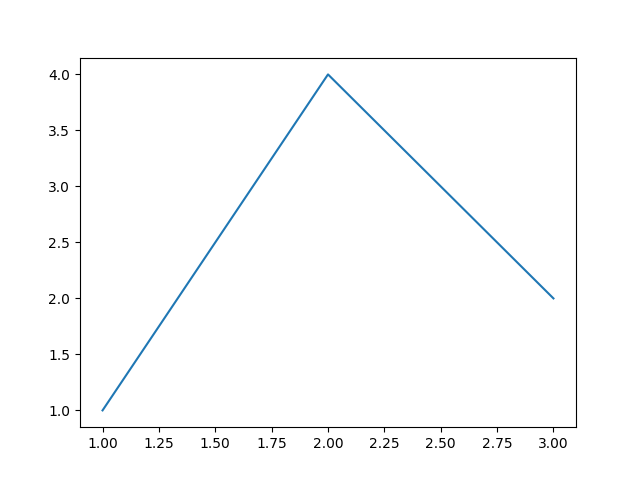
\includegraphics[scale=0.35]{code_04/41.png}
\end{frame}


\begin{frame}{Заголовок, подписи, легенда}
\lstinputlisting[language=Python]{code_04/42_1.py}
\vspace{0cm}
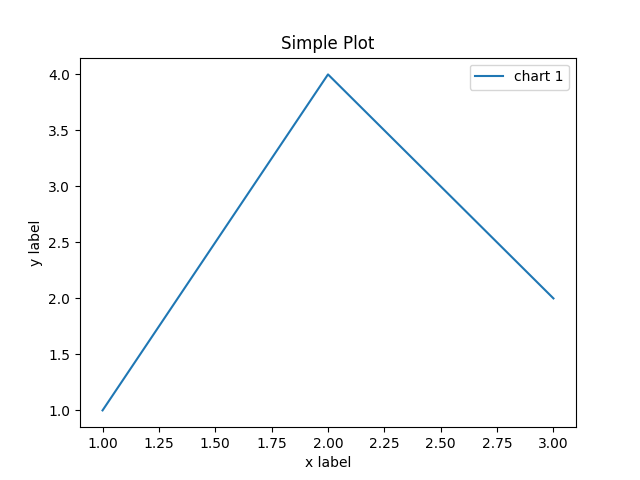
\includegraphics[scale=0.35]{code_04/42.png}
\end{frame}

\begin{frame}{Два и более графиков}
\lstinputlisting[language=Python]{code_04/43_1.py}
\vspace{0cm}
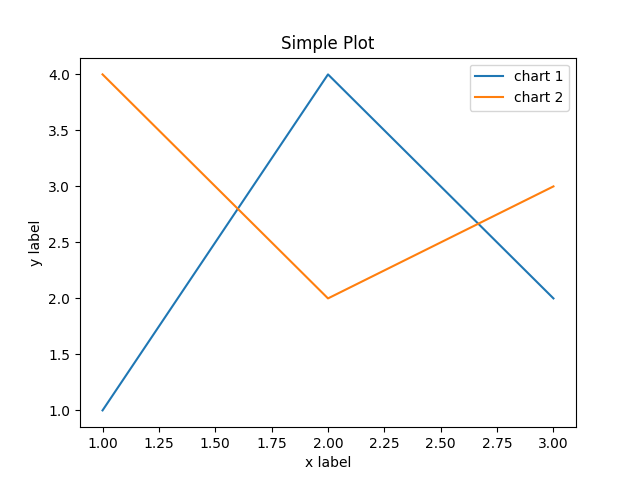
\includegraphics[scale=0.35]{code_04/43.png}
\end{frame}

\begin{frame}{Сетка}
\lstinputlisting[language=Python]{code_04/44_1.py}
\vspace{0cm}
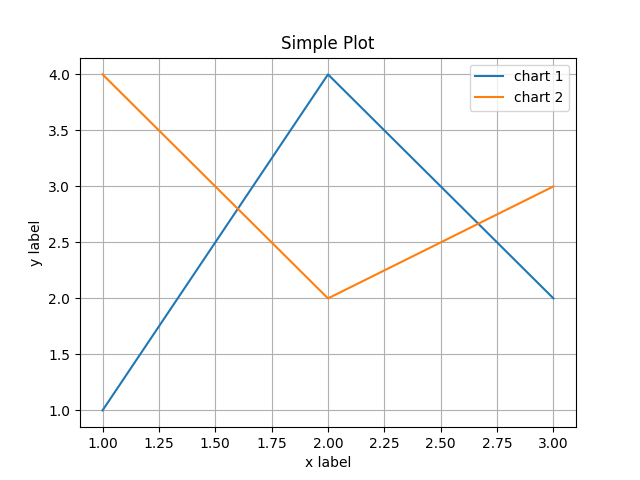
\includegraphics[scale=0.35]{code_04/44.png}
\end{frame}


\section{Математическая библиотека numpy}
\begin{frame}[t]{Оглавление}
\tableofcontents[currentsection]
\end{frame}

\subsection{Установка библиотеки}
\begin{frame}{Библиотека numpy}
\textbf{\# Установка библиотеки numpy} \\
\vspace{0.5cm}
pip install numpy \\
\vspace{0.2cm}
pip install scipy
\end{frame}


\begin{frame}{График функции y = sin(x)}
\lstinputlisting[language=Python]{code_04/45.py}
\end{frame}


\begin{frame}{Матрицы}
\textbf{Матрицей} в математике называют объект, записываемый в виде прямоугольной таблицы, элементами которой являются числа (могут быть как действительные, так и комплексные). \\
\vspace{0.5cm}
\[
  A_{3\times 3} = 
  \begin{pmatrix}
    a_{11} & a_{12} & a_{13}\\
    a_{21} & a_{22} & a_{23}\\
    a_{31} & a_{32} & a_{33}
  \end{pmatrix}
\]

\begin{itemize}
\item Матрица состоит из i-строк и j-столбцов;
\item Каждый ее элемент имеет соответствующее позиционное обозначение: $a_{ij}$ находится на \emph{i}-ой строке и \emph{j}-м столбце;
\item Главная диагональ -- элементы, у которых совпадают номера строк и столбцов.
\end{itemize}
\end{frame}

\subsection{Вектор}
\begin{frame}{Вектор}
\textbf{Вектором} называется матрица, у которой есть только один столбец или одна строка. \\
\vspace{0.5cm}
Вектор-строка имеет следующую математическую запись
\vspace{0.2cm}
\[
  v = 
  \begin{pmatrix}
    a_{11} & a_{12} \\
  \end{pmatrix}
\]
\\
\vspace{0.2cm}
в Python можно задать следующим образом
\vspace{0.2cm}
\lstinputlisting[language=Python]{code_04/47.py}
\vspace{0.2cm}
Результат: \\
\lstinputlisting[language=Python]{code_04/47_1.txt}
\end{frame}


\begin{frame}{Вектор}
Вектор-столбец имеет следующую математическую запись
\vspace{0.2cm}
\[
  v = 
  \begin{pmatrix}
    a_{11}\\
    a_{21}\\
  \end{pmatrix}
\]
\\
\vspace{0.2cm}
в Python можно задать следующим образом
\vspace{0.2cm}
\lstinputlisting[language=Python]{code_04/48.py}
\vspace{0.2cm}
Результат: \\
\lstinputlisting[language=Python]{code_04/48_1.txt}
\end{frame}


\subsection{Квадратная матрица}
\begin{frame}{Квадратная матрица}
Матрица называется \textbf{квадратной}, если количество строк и столбцов совпадают.
\vspace{0.2cm}
\[
  v = 
  \begin{pmatrix}
    1 & 2 & 3 \\
    4 & 5 & 6 \\
    7 & 8 & 9 \\
  \end{pmatrix}
\]
\\
%\vspace{0.2cm}
\lstinputlisting[language=Python]{code_04/49.py}
%\vspace{0.2cm}
Результат: \\
\lstinputlisting[language=Python]{code_04/49_1.txt}
\end{frame}


\subsection{Диагональная матрица}
\begin{frame}{Диагональная матрица}
\textbf{Диагональная матрица} – матрица, у которой все элементы, кроме тех, что расположены на главной диагонали, равны нулю.
\vspace{0.2cm}
\[
  v = 
  \begin{pmatrix}
    1 & 0 & 0 \\
    0 & 5 & 0 \\
    0 & 0 & 9 \\
  \end{pmatrix}
\]
\\
%\vspace{0.2cm}
\lstinputlisting[language=Python]{code_04/50.py}
%\vspace{0.2cm}
Результат: \\
\lstinputlisting[language=Python]{code_04/50_1.txt}
\end{frame}

\subsection{Единичная матрица}
\begin{frame}{Единичная матрица}
\textbf{Единичной матрицей} называют такую квадратную матрицу, у которой элементы главной диагонали равны единицы, а все остальные нулю.
\vspace{0.2cm}
\[
  v = 
  \begin{pmatrix}
    1 & 0 & 0 \\
    0 & 1 & 0 \\
    0 & 0 & 1 \\
  \end{pmatrix}
\]
\\
\vspace{-0.6cm}
\lstinputlisting[language=Python]{code_04/51.py}
%\vspace{0.2cm}
Результат: \\
\lstinputlisting[language=Python]{code_04/51_1.txt}
\end{frame}


\subsection{Сложение матриц}
\begin{frame}{Сложение матриц A + B}
\[
  A = 
  \begin{pmatrix}
    a_{11} & a_{12} & a_{13}\\
    a_{21} & a_{22} & a_{23}\\
    a_{31} & a_{32} & a_{33}
  \end{pmatrix}
\]
\\
\[
  B = 
  \begin{pmatrix}
    b_{11} & b_{12} & b_{13}\\
    b_{21} & b_{22} & b_{23}\\
    b_{31} & b_{32} & b_{33}
  \end{pmatrix}
\]
\\
Сложение матриц
\\
\[
  A + B = 
  \begin{pmatrix}
    a_{11} + b_{11} & a_{12} + b_{12} & a_{11} + b_{13}\\
    a_{21} + b_{21} & a_{22} + b_{22} & a_{23} + b_{23}\\
    a_{31} + b_{31} & a_{32} + b_{32} & a_{33} + b_{33}
  \end{pmatrix}
\]
\end{frame}


\begin{frame}{Сложение матриц A + B}
\lstinputlisting[language=Python]{code_04/53.py}
%\vspace{0.2cm}
Результат: \\
\lstinputlisting[language=Python]{code_04/53_1.txt}
\end{frame}


\subsection{Вычитание матриц}
\begin{frame}{Вычитание матриц A - B}
\[
  A = 
  \begin{pmatrix}
    a_{11} & a_{12} & a_{13}\\
    a_{21} & a_{22} & a_{23}\\
    a_{31} & a_{32} & a_{33}
  \end{pmatrix}
\]
\\
\[
  B = 
  \begin{pmatrix}
    b_{11} & b_{12} & b_{13}\\
    b_{21} & b_{22} & b_{23}\\
    b_{31} & b_{32} & b_{33}
  \end{pmatrix}
\]
\\
Вычитание матриц
\\
\[
  A - B = 
  \begin{pmatrix}
    a_{11} - b_{11} & a_{12} - b_{12} & a_{11} - b_{13}\\
    a_{21} - b_{21} & a_{22} - b_{22} & a_{23} - b_{23}\\
    a_{31} - b_{31} & a_{32} - b_{32} & a_{33} - b_{33}
  \end{pmatrix}
\]
\end{frame}


\begin{frame}{Вычитание матриц A - B}
\lstinputlisting[language=Python]{code_04/54.py}
%\vspace{0.2cm}
Результат: \\
\lstinputlisting[language=Python]{code_04/54_1.txt}
\end{frame}


\subsection{Скалярное произведение}
\begin{frame}{Скалярное произведение A $*$ n}
В скалярном произведении постоянное значение умножается на каждый элемент матрицы.\\
\[
  A = 
  \begin{pmatrix}
    a_{11} & a_{12} & a_{13}\\
    a_{21} & a_{22} & a_{23}\\
    a_{31} & a_{32} & a_{33}
  \end{pmatrix}
\]
\\
Умножения матрицы А на число \emph{n}
\\
\[
  A \times n = 
  \begin{pmatrix}
    a_{11} \times n & a_{12} \times n & a_{11} \times n \\
    a_{21} \times n & a_{22} \times n & a_{23} \times n \\
    a_{31} \times n & a_{32} \times n & a_{33} \times n
  \end{pmatrix}
\]
\end{frame}


\begin{frame}{Скалярное произведение  A $*$ n}
Оператор $*$ используется для умножения скалярного значения на элементы входной матрицы.
\vspace{0.2cm}
\lstinputlisting[language=Python]{code_04/55.py}
%\vspace{0.2cm}
Результат: \\
\lstinputlisting[language=Python]{code_04/55_1.txt}
\end{frame}




\subsection{Произведение матриц}
\begin{frame}{Произведение матриц}
Каждый элемент результирующей матрицы — сумма произведений каждого элемента соответствующей строки в первой матрице с соответствующим элементом из колонки второй. 
\vspace{0.2cm}
\center{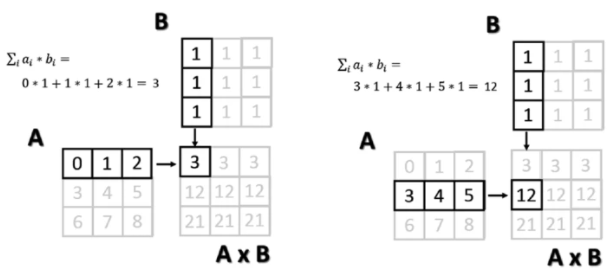
\includegraphics[scale=0.4]{image/matrix_dot.png}} \\
\end{frame}


\begin{frame}{Произведение матриц numpy.dot(A, B)}
\lstinputlisting[language=Python]{code_04/52.py}
%\vspace{0.2cm}
Результат: \\
\lstinputlisting[language=Python]{code_04/52_1.txt}
\end{frame}



\part{2}

\begin{frame}[t]{Литература}
\setbeamertemplate{bibliography item}[text]

\begin{thebibliography}{3}

\bibitem{src_this}
Презентация [Лекции 01-04] \\
\vspace{0.2cm}
\textit{\href{https://github.com/IRyazantsev/mpei_python_mini-course_2021/tree/main/bin}{https://github.com/IRyazantsev/mpei\_python\_mini-course\_2021/tree/main/bin}}

\bibitem{texbook}
Python 3. Самое необходимое | Дронов В.А., Прохоренок Н.А.

\bibitem{texbook} 
Изучаем Python. Том 1, 2 | Лутц Марк

\bibitem{texbook} 
Python 3 и PyQt 5. Разработка приложений | Прохоренок Н.А., Дронов В.А.

\bibitem{texbook} 
Django 3.0. Практика создания веб-сайтов на Python | Дронов В. А.

\bibitem{texbook} 
Разработка веб-приложений с использованием Flask | Гринберг Мигель

\end{thebibliography}
\end{frame}


\begin{frame}[t]{Вопросы}
\vspace{0.7cm}
\center{
\includegraphics[scale=0.3]{image/questions.jpg}} \\
\end{frame}

\end{document}